\documentclass[aps,prl,twocolumn,superscriptaddress,longbibliography]{revtex4-2}

\usepackage{amssymb}
\usepackage{amsmath}
\usepackage[utf8]{inputenc}
\usepackage{array}
\usepackage{multirow}
\usepackage{color}
\usepackage{esint}
\usepackage{bm}
\usepackage{color}
\usepackage{bbm}
\usepackage{babel}
\usepackage{titlesec}
\usepackage{graphicx,amssymb,color}
\usepackage{epsfig}
\usepackage{epstopdf}
\usepackage{mathtools}
\usepackage{soul}
\usepackage[dvipsnames]{xcolor}
\usepackage{tikz}
\usepackage{tcolorbox}
\usepackage{graphics,amssymb,amsmath,epsfig,color}
\usepackage{physics}
\usepackage[breaklinks,colorlinks,
linkcolor=violet,citecolor=violet,urlcolor=violet]{hyperref}
\usepackage{orcidlink}

% \usepackage{amsmath,amssymb,bm}
% \usepackage{graphicx}
% \usepackage{hyperref}
% \usepackage{xcolor}
% \usepackage{orcidlink}

\newcommand{\br}{\mathbf{r}}
\newcommand{\bv}{\mathbf{v}}
\newcommand{\bx}{\mathbf{X}}
\newcommand{\avg}[1]{\langle #1 \rangle}

\begin{document}

\title{From variational Monte Carlo to superfluid hydrodynamics\\
in microwave-shielded Bose Einstein condensates}

\author{Xin-Yuan Gao\orcidlink{0000-0003-0608-9029}}
\thanks{These authors contributed equally.}
\affiliation{%
Department of Physics, The Chinese University of Hong Kong, Shatin, New Territories, Hong Kong, China
}%
\author{Kai Yuen Lee\orcidlink{0009-0005-9491-0340}}
\thanks{These authors contributed equally.}
\affiliation{%
Department of Physics, The Chinese University of Hong Kong, Shatin, New Territories, Hong Kong, China
}%
\author{Yangqian Yan\orcidlink{0000-0002-3237-5945}}%
\email{yqyan@cuhk.edu.hk}
\affiliation{%
Department of Physics, The Chinese University of Hong Kong, Shatin, New Territories, Hong Kong, China
}
\affiliation{State Key Laboratory of Quantum Information Technologies and Materials, The Chinese University of Hong Kong, Hong Kong SAR, China}
\affiliation{
The Chinese University of Hong Kong Shenzhen Research Institute, 518057 Shenzhen, China
}%

\date{\today}

\begin{abstract}
We show that, within the manifold where the Jastrow pair factor is
frozen to its ground-state form, time-dependent variational Monte Carlo
(tVMC) based on a Jastrow--Feenberg wavefunction maps exactly onto
irrotational superfluid hydrodynamics.  The only microscopic input is
an equation of state (EOS) extracted from a single variational Monte
Carlo calculation of the uniform system, which yields a
density-dependent chemical potential $\mu(\rho)$ for a generalized
Gross--Pitaevskii equation (GPE).  For a trapped microwave-shielded
dipolar Bose gas, this reduced description reproduces the full tVMC
breathing dynamics for $N=8$--$128$ with below-1\% frequency error and
$\sim 2\%$ amplitude error, while lowering the computational cost by
more than an order of magnitude.  The framework turns correlated tVMC
into a practical predictive tool for collective dynamics in shielded
molecular gases.
\end{abstract}

\maketitle

%======================================================================
\emph{Introduction.}---Microwave-shielded polar molecules have emerged
as a promising platform for quantum many-body physics, with recent
experiments achieving Bose--Einstein condensation~\cite{Bigagli2024},
observing shielded collisions~\cite{Anderegg2021,Schuster2023}, and
probing dipolar many-body effects~\cite{Karman2018,Karman2019,Chen2023}.
A central theoretical challenge is to predict nonequilibrium collective
dynamics---breathing oscillations, quenches, and expansion---from the
microscopic interaction, which combines long-range dipolar attraction
($\sim C_3/r^3$) with short-range repulsive shielding ($\sim C_6/r^6$).

Mean-field Gross--Pitaevskii (GP) theory is computationally efficient
but reduces this interaction to a contact nonlinearity, thereby missing
the anisotropic and density-dependent correlations generated by the
shielding mechanism.  At the opposite end, time-dependent variational
Monte Carlo (tVMC)~\cite{Carleo2012,Carleo2014} can treat realistic
interactions within a correlated many-body wavefunction, but its
stochastic sampling at every time step severely limits accessible system
sizes and evolution times.

This Letter introduces a general theoretical framework that retains the
microscopic content of tVMC while recovering the efficiency of
hydrodynamics. While demonstrated here for shielded molecular gases,
this approach provides a pathway for describing collective dynamics in
other strongly correlated fluids, such as quantum droplets, supersolids,
and strongly interacting Rydberg gases, where standard mean-field theories
often break down. Our central result is conditional but exact: once the
two-body Jastrow factor $u_2$ is frozen, the time-dependent variational
principle (TDVP) maps exactly onto irrotational superfluid hydrodynamics.
We first verify from full tVMC that $u_2$ remains nearly stationary during
the quench, then extract the uniform-system EOS from a one-time VMC calculation,
and finally solve a generalized GPE with this EOS. The resulting dynamics
reproduces the full tVMC benchmarks for $N=8$ and $N=128$ and extends
straightforwardly to experimentally relevant large-$N$ regimes beyond direct tVMC.

%======================================================================
\emph{Model and variational dynamics.}---We consider $N$ bosons in a
cylindrically symmetric harmonic trap with Hamiltonian
\begin{equation}
\hat{H}(t) = \sum_{i=1}^N\!\left[
-\tfrac{1}{2}\nabla_i^2 + V_{\mathrm{tr}}(\br_i,t)\right]
+ \sum_{i<j} v(\br_{ij}),
\label{eq:H}
\end{equation}
where $V_{\mathrm{tr}} = \frac{1}{2}[\omega_\rho(t)^2\rho^2 +
\omega_z^2 z^2]$ (natural units $\hbar=m=1$) and the two-body
interaction models microwave-shielded dipolar molecules:
\begin{equation}
v(\br) = \frac{C_3}{r^3}(3\cos^2\!\theta-1)
+ \frac{C_6}{r^6}(\sin^4\!\theta + w_{12}\sin^2\!\theta\cos^2\!\theta).
\label{eq:V}
\end{equation}
This effective potential, derived from Floquet scattering theory for
dual-microwave-dressed molecules~\cite{Deng2025}, is parametrized by
coefficients $C_3$, $C_6$, and $w_{12}$ that are determined by the
microwave field configuration.  In a realistic experiment these are
fixed by the dressing scheme; here, for demonstration, we choose
$C_3=10^{-3}$, $C_6=10^{-6}$, and $w_{12}=2.0$ in oscillator units.
We study a quench $\omega_\rho: 1\to 2$ at $t=0$ that excites radial
breathing modes.

The many-body wavefunction is a truncated
Jastrow--Feenberg~\cite{Jastrow1955,Feenberg1969} ansatz:
\begin{equation}
\Psi(\bx,t) = \exp\!\Big[\sum_i u_1(\br_i,t)
+ \sum_{i<j} u_2(r_{ij},\hat\br_{ij})\Big],
\label{eq:Psi}
\end{equation}
where $u_1(\br,t)$ is a complex, time-dependent one-body field and
$u_2$ encodes two-body correlations.  In cylindrical geometry we use a
separable parametrization for $u_1$, while $u_2$ is expanded in partial
waves as
\begin{equation}
u_2(r,\cos\theta) = u_{\mathrm{cusp}}(r) + \sum_{\ell=0,2,4}
f_\ell(r)\,P_\ell(\cos\theta),
\label{eq:u2}
\end{equation}
where $u_{\mathrm{cusp}}(r)$ captures the short-range scattering
boundary condition and each $f_\ell$ is represented by Gaussian basis
functions~\cite{SM_note}.  For the parameters studied here, the
$\ell=4$ channel is negligible and the $\ell=2$ anisotropy is weak, so
the pair correlation is close to isotropic.

Figure~\ref{fig:hnc} shows the quality of the optimized pair
correlations.  The leading-order hypernetted-chain (HNC) approximation
to the pair distribution function, $g_2^{\mathrm{HNC}}(r,\theta) =
e^{2u_2(r,\cos\theta)}$~\cite{Hansen2006}, reveals a correlation hole
at short range [Fig.~\ref{fig:hnc}(a)], reflecting the interplay between
dipolar attraction along $\theta=0$ and the shielding repulsion.  The
pair correlation is nearly isotropic, consistent with the subdominant
role of $f_2$.

\begin{figure}[t]
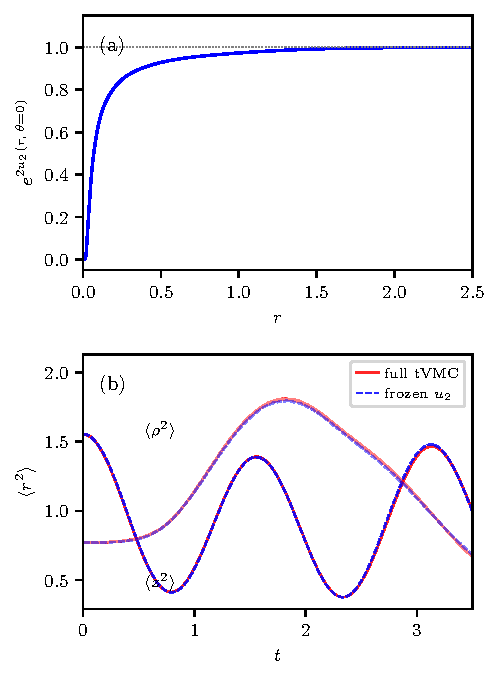
\includegraphics[width=\columnwidth]{fig1_hnc_dynamics.pdf}
\caption{(a)~Leading-order HNC pair correlation
$e^{2u_2(r,\theta{=}0)}$ for the $N{=}8$ ground state, showing a
correlation hole at short range due to the shielding repulsion.
(b)~Breathing dynamics after the quench $\omega_\rho:1\to 2$ for
$N{=}128$: $\avg{\rho^2}(t)$ and $\avg{z^2}(t)$ from full tVMC (red)
and frozen-$u_2$ tVMC (blue dashed), validating the frozen-$u_2$
approximation.}
\label{fig:hnc}
\end{figure}

The TDVP~\cite{Dirac1930,McLachlan1964} projects the Schr\"odinger
equation onto the variational tangent space.  Defining logarithmic
derivatives $O_\alpha =
\partial_{\theta_\alpha}\ln\Psi$ and the local energy
$E_L = (\hat{H}\Psi)/\Psi$, the equations of motion
read~\cite{Carleo2012}
\begin{equation}
\sum_\beta S_{\alpha\beta}\,\dot\theta_\beta = -i\,F_\alpha,
\label{eq:tdvp}
\end{equation}
where the overlap matrix and force vector are
\begin{align}
S_{\alpha\beta} &= \avg{\Delta O_\alpha^*\,\Delta O_\beta}_t,
\label{eq:S}\\
F_\alpha &= \avg{\Delta O_\alpha^*\,\Delta E_L}_t,
\label{eq:F}
\end{align}
with $\Delta A = A - \avg{A}_t$ denoting connected fluctuations.  Full
Monte Carlo and convergence details are given in Ref.~\cite{SM_note}.

%======================================================================
\emph{Frozen-$u_2$ reduction.}---The key numerical observation is that
during the quench the optimized two-body parameters change by less than
$1\%$ of their ground-state values, while the one-body field changes by
order unity.  Figure~\ref{fig:hnc}(b) already shows that a frozen-$u_2$
tVMC evolution tracks the full tVMC dynamics, and
Fig.~\ref{fig:u2_heatmap} visualizes the near-stationarity of the pair
correlation itself.  This motivates restricting the variational
manifold to a fixed $u_2$.

When the variational degree of freedom is the continuous field
$u_1(\br,t)$, the TDVP logarithmic derivative becomes the microscopic
density operator:
\begin{equation}
O(\br;\bx) = \frac{\delta\ln\Psi}{\delta u_1(\br)}
= \sum_i\delta^{(3)}(\br-\br_i) = \hat\rho(\br).
\label{eq:O_rho}
\end{equation}
Because $u_2$ is real and frozen, the many-body phase is purely one-body
and irrotational: $\bv = \nabla(\mathrm{Im}\, u_1)$.  No backflow terms
arise.

Decomposing $u_1 = a + i\theta$ (real amplitude and phase), the TDVP
action reduces to the standard hydrodynamic form~\cite{SM_note}.  Within
this frozen-$u_2$ manifold the reduction is exact and yields
the continuity and Euler equations:
\begin{align}
&\partial_t\rho + \nabla\!\cdot(\rho\bv) = 0,
\label{eq:cont}\\
&\partial_t\bv + \nabla\!\Big(\tfrac{1}{2}v^2 + V_{\mathrm{tr}}
+ \mu_{u_2}[\rho]\Big) = 0,
\label{eq:euler}
\end{align}
where $\mu_{u_2}[\rho] = \delta E_{\mathrm{int}}[\rho;u_2]/\delta\rho$
is the effective chemical potential determined by the frozen correlations.

To obtain a closed local theory, we further invoke the local-density
approximation (LDA).  The internal energy then takes the
form $E_{\mathrm{int}} = \int\!\rho\,\varepsilon(\rho)\,d^3r$, where
$\varepsilon(\rho)$ is the energy per particle of the \emph{uniform}
system at density $\rho$ with the same frozen $u_2$.  The chemical
potential becomes a local function:
\begin{equation}
\mu(\rho) = \frac{d[\rho\varepsilon(\rho)]}{d\rho}
= \varepsilon + \rho\varepsilon'.
\label{eq:mu}
\end{equation}
This is structurally identical to GP theory, except that the usual
contact coupling $gn$ is replaced by $\mu(\rho)$, which encodes the
full effect of the realistic, anisotropic interaction through the
frozen correlations.

The near-stationarity of $u_2$ during the quench is visualized
directly in Fig.~\ref{fig:u2_heatmap}, which shows the change in the
leading-order HNC pair correlation $\Delta e^{2u_2}$ at four time
snapshots.  The variation remains below $\sim 0.03$ throughout
(compared to peak values $\sim 1$), confirming that the pair
correlations are effectively frozen.

\begin{figure*}[t]
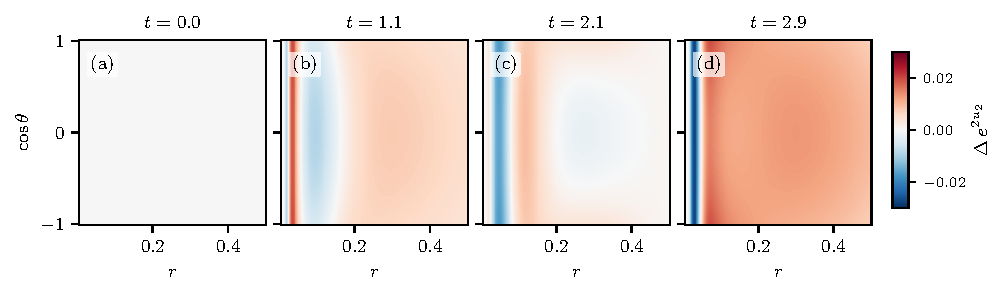
\includegraphics[width=\textwidth]{fig2_u2_heatmap.pdf}
\caption{Change in the leading-order HNC pair correlation,
$\Delta e^{2u_2} = e^{2u_2(t)} - e^{2u_2(0)}$, during breathing
dynamics for $N{=}128$.  The pair correlations remain nearly frozen
($|\Delta e^{2u_2}| \lesssim 0.03$) while the one-body density
undergoes order-unity changes.}
\label{fig:u2_heatmap}
\end{figure*}

%======================================================================
\emph{Equation of state and generalized GPE.}---We extract
$\varepsilon(\rho)$ from a one-time VMC calculation on the
uniform system (periodic boundary conditions) with $u_2$ frozen at its
trapped ground-state values.  Scanning 20--30 density values
logarithmically from $\rho=0.05$ to $\rho_{\max}$ (3.0 for $N=8$;
15.0 for $N=128$) with 8192 walkers, we fit the results to
\begin{equation}
\varepsilon(\rho) = a_1\rho + a_2\rho^2 + \cdots,
\label{eq:eos}
\end{equation}
yielding the chemical potential
$\mu(\rho) = 2a_1\rho + 3a_2\rho^2+\cdots$.

This expansion gives a compact physical interpretation of the EOS.
Relative to the standard GPE nonlinearity $\mu = g\rho$, the leading term
$2a_1\rho$ corresponds to a \emph{renormalized two-body coupling}
$g_{\mathrm{eff}} = 2a_1$, which absorbs the effect of the frozen
pair correlations into an effective contact interaction.  The
next-order term $3a_2\rho^2$, however, has the structure of an
\emph{effective three-body interaction} with coupling strength
$g_3 = 3a_2$.  This is not a genuine microscopic three-body force;
rather, it emerges from integrating out the density dependence of the
two-body correlations encoded in $u_2$.  In density-functional
language, it is the leading beyond-mean-field correction to the
interaction energy~\cite{PitaevskiiStringari2016}.

For the shielded dipolar interaction studied here, we find
$g_3/g_{\mathrm{eff}}^2 \sim 0.1$--$0.2$, indicating that the
three-body term provides a 10--20\% correction at the equilibrium
density.  For $N=8$, the data require a weak cubic correction, whereas
for $N=128$ a quadratic fit with $a_1{=}0.111$ and $a_2{=}0.001$
already describes the relevant density range and remains stable
($d\mu/d\rho > 0$).  The EOS is therefore close to linear at high
density, reflecting the long-range character of the shielded dipolar
interaction.

The VMC EOS for two interaction strengths is shown in
Fig.~\ref{fig:eos}.  The leading coefficient $a_1$ scales linearly with
$C_3$, while $a_2$ captures the density-dependent beyond-mean-field
corrections.

\begin{figure}[t]
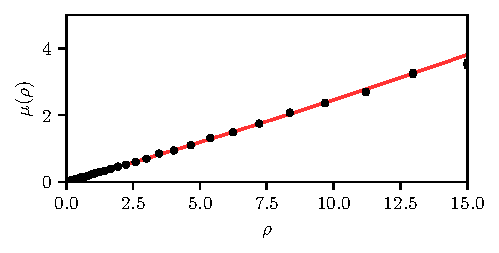
\includegraphics[width=\columnwidth]{fig3_eos.pdf}
\caption{Chemical potential $\mu(\rho)=d(\rho\varepsilon)/d\rho$ from
uniform-system VMC for $C_3{=}10^{-3}$ (circles, black fit) and
$C_3{=}10^{-4}$ (squares, red fit).  Data points are obtained by
numerical differentiation of the VMC energy; lines show polynomial
fits used in the GPE.}
\label{fig:eos}
\end{figure}

The resulting generalized GPE,
\begin{equation}
i\partial_t\psi = \Big[-\tfrac{1}{2}\nabla^2
+ V_{\mathrm{tr}} + g_{\mathrm{eff}}|\psi|^2
+ g_3|\psi|^4\Big]\psi,
\label{eq:gpe_g3}
\end{equation}
is therefore a \emph{two-plus-three-body} GPE whose couplings are fixed
microscopically by VMC rather than by phenomenology.  This provides a
first-principles realization of the extended GPE forms discussed in the
contexts of quantum droplets~\cite{Petrov2015} and dipolar
condensates~\cite{Chomaz2023,Lahaye2009}.

%======================================================================
\emph{GPE solver.}---We solve the generalized GPE
\begin{equation}
i\partial_t\psi = \Big[-\tfrac{1}{2}\nabla^2
+ V_{\mathrm{tr}} + \mu(|\psi|^2)\Big]\psi,
\label{eq:gpe}
\end{equation}
where $\psi = \sqrt\rho\,e^{i\theta}$ and the Laplacian provides both
quantum pressure and flow kinetic energy.  The equation is discretized
on a cylindrical $(r,z)$ grid exploiting azimuthal symmetry, with a
fourth-order finite-difference Laplacian (including L'H\^opital's rule
at $r=0$) and fourth-order Runge--Kutta time integration under a
dispersive CFL condition $\Delta t \leq C\Delta x^2/\pi$
($C=0.3$)~\cite{SM_note}.

The initial state is obtained by imaginary-time propagation to
self-consistency: $\psi \to \psi - d\tau\,\hat H\psi$, normalized to
$N$ particles at each step, until the chemical potential converges to
$\delta\mu < 10^{-8}$.

%======================================================================
\emph{Validation against tVMC.}---We benchmark the generalized GPE
against frozen-$u_2$ tVMC at both weak and moderate interaction
strength.  For $N=8$, the GPE ground state reproduces the tVMC moments
to 0.7\% and the energy to 0.15\% (Table~S1~\cite{SM_note}).  The
breathing frequency is $\omega_{\mathrm{br}} = 4.19 \approx 2\omega_\rho$
in both methods, and the oscillation amplitudes of $\avg{\rho^2}$ and
$\avg{z^2}$ agree to within 1\%.  The quantum-pressure term is essential
in this regime because the interaction energy is only $\sim 3.5\%$ of
the total.

For $N=128$, where the interaction energy reaches $\sim 21\%$ of the
total, the same EOS-based GPE remains accurate.  The ground-state
moments agree with tVMC to $0.35\%$ for $\avg{\rho^2}$ and $1.05\%$ for
$\avg{z^2}$, while the total energy differs by 2.8\%, consistent with a
residual LDA error at higher density.  More importantly, the dynamical
benchmark in Fig.~\ref{fig:dynamics}(a) is essentially unchanged:
$\omega_{\mathrm{br}} = 4.19$ in both approaches and the
$\avg{\rho^2}(t)$ amplitude agrees to $\sim 2\%$.

The computational gain is substantial.  For $N=128$, the GPE evolution
including imaginary-time state preparation takes $\sim 70$ minutes on a
single CPU core, compared with $\sim 6$ hours on a modern GPU for the
full tVMC.  The reduction is larger still in total floating-point cost,
since the stochastic tVMC evolution requires fresh Monte Carlo sampling
at every Runge--Kutta stage.

\emph{Large-$N$ prediction.}---Having benchmarked the reduction, we use
it in a regime inaccessible to direct tVMC.  For a weaker interaction,
$C_3 = 10^{-4}$, the VMC-derived EOS predicts sustained breathing
oscillations for $N=10{,}000$ over at least ten trap periods
[Fig.~\ref{fig:dynamics}(b)].  This illustrates the practical value of
the approach: once the EOS is known, the many-body quench problem is
reduced to a deterministic hydrodynamic evolution.

\begin{figure}[t]
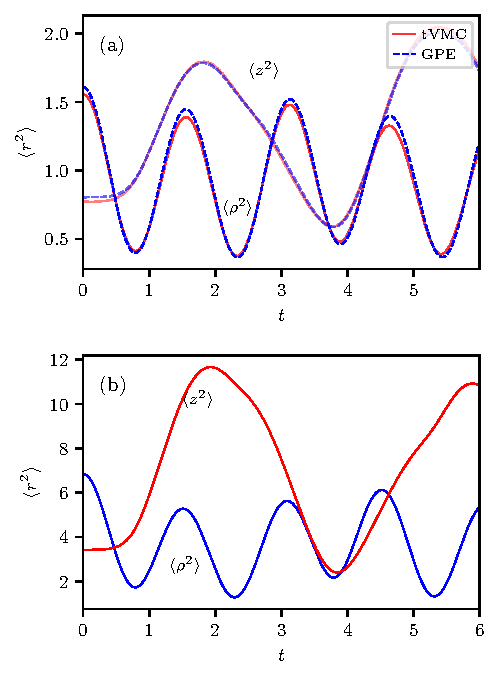
\includegraphics[width=\columnwidth]{fig4_dynamics.pdf}
\caption{GPE dynamics from the VMC-derived EOS.
(a)~$N{=}128$ validation: $\avg{\rho^2}(t)$ and $\avg{z^2}(t)$ from
frozen-$u_2$ tVMC (red) and GPE (blue), showing identical breathing
frequencies within numerical resolution.
(b)~$N{=}10{,}000$ prediction with the weak-interaction EOS
($C_3{=}10^{-4}$), extrapolating to experimentally relevant system
sizes inaccessible to direct tVMC.}
\label{fig:dynamics}
\end{figure}

%======================================================================
\emph{Discussion.}---The success of the frozen-$u_2$ hydrodynamic
reduction rests on a physical separation of scales: short-range pair
correlations, governed by the interaction potential on lengths
$r\lesssim a_{\mathrm{ho}}$, equilibrate much faster than the global
density redistribution driven by the trap quench.  This is manifested
in the tVMC as $<1\%$ variation of the $u_2$ parameters during the
quench, while $u_1$ changes by order unity.

Two features distinguish the present framework from standard GP theory.
First, the EOS is microscopically derived from the correlated many-body
wavefunction rather than inferred from a scattering-length reduction.
Second, the hydrodynamic equation is not postulated: it follows directly
from the TDVP once the dynamics is projected onto the frozen-$u_2$
manifold.  In this sense, the approximation is transparent and
diagnosable: its validity can be checked a posteriori by monitoring the
time dependence of $u_2$.

The same construction also clarifies the origin of higher-order
nonlinearities.  The effective three-body term $g_3|\psi|^4$ in
Eq.~\eqref{eq:gpe_g3} is not inserted phenomenologically; it emerges
from the density dependence of correlated two-body physics.  This makes
the method a useful nonperturbative route to extended GPEs for dipolar
and molecular systems, where beyond-mean-field effects are often
important but difficult to parameterize reliably.

The main quantitative limitation visible here is the $\sim 3\%$ energy
offset at $N=128$, which points to gradient corrections beyond the
LDA~\cite{Ancilotto2017}.  More generally, the present reduction should
hold when pair correlations remain slaved to the evolving density and
the flow stays irrotational.  It can then be extended naturally to other
collective modes, quench protocols, and trap geometries relevant to
current molecular-gas experiments~\cite{Bigagli2024,Lin2024}.

%======================================================================
\emph{Conclusion.}---We have demonstrated that correlated many-body
dynamics from tVMC maps exactly onto superfluid hydrodynamics within the
frozen-$u_2$ manifold, with the required equation of state obtained from
a single uniform-system VMC calculation. The resulting generalized GPE
reproduces the breathing dynamics of microwave-shielded dipolar bosons
from $N=8$ to $N=128$ with below-1\% frequency error and $\sim 2\%$
amplitude error, while providing access to large-$N$ regimes beyond
direct tVMC. Beyond establishing a practical bridge between microscopic
physics and predictive hydrodynamics for molecular gases, the ``frozen-Jastrow''
hydrodynamic concept introduced here establishes a powerful methodology.
It has the potential to enable first-principles modeling of non-equilibrium
dynamics in a wide array of quantum fluids governed by complex long- and
short-range correlations, including quantum droplets, supersolids, and
Rydberg atomic gases.

\begin{acknowledgments}
Computations were performed using JAX~\cite{Bradbury2018} for
GPU-accelerated VMC.
We would like to acknowledge financial support from the National Natural Science Foundation of China under Grant No. 124B2074 and No. 12204395, Hong Kong RGC Early Career Scheme (Grant No. 24308323) and Collaborative Research Fund (Grant No. C4050-23GF), the Space Application System of China Manned Space Program, Guangdong Provincial Quantum Science Strategic Initiative GDZX2404004, and CUHK Direct Grant No. 4053731.
\end{acknowledgments}

\bibliography{letter_refs}

\end{document}
